\documentclass[runningheads]{llncs}

\usepackage[T1]{fontenc}
\usepackage{amsmath,amssymb}
\usepackage{graphicx}
\usepackage{booktabs}
\usepackage{algorithm}
\usepackage{algpseudocode}
\usepackage{tikz}
\usetikzlibrary{positioning,arrows.meta}
\usepackage{pgfplots}
\pgfplotsset{compat=1.16}

\begin{document}

\title{CETP: Cross-Environment Runtime Prediction for PostgreSQL Queries}

\titlerunning{CETP: Cross-Environment Runtime Prediction for PostgreSQL Queries}

\author{Harshith J \and Sarthak Wadhwa \and Kartik Bhat Sumbly \and
Ishanvee Amit Sinha \and Dr. Nivedita Kasturi}

\authorrunning{Harshith J et al.}

\institute{Department of Computer Science and Engineering, PES University,
Bangalore, India\\
\email{harshithj@gmail.com, sarthakwadhwa@gmail.com, kartikbhat@gmail.com,
ishanveesinha@gmail.com, niveditak@pes.edu}}

\maketitle

\begin{abstract}
A query that is fast on a developer's laptop can be slow on the production
server, and the developer usually finds out after deployment. We present CETP
(Cross-Environment Runtime Prediction), which estimates the production runtime
of a PostgreSQL query from a plan captured on the developer's own machine.
Each machine is described by running PostgreSQL's own operators in SQL: five
serial rates (sequential scan, hash join, sort, hash aggregation and nested
loop) and the speedup the machine actually delivers to a parallel scan. The
development runtime is then scaled operator by operator, with the parallel
term applied only to the part of the plan that runs under a Gather node. We
evaluate on all 22 TPC-H queries across thirteen environments and two
instruction sets. On a grid of eight containers with independently varied CPU
and memory limits, the model reaches 22.41\% mean absolute percentage error
against 72.52\% for assuming production equals development. From a laptop to
seven same-architecture targets it scores 29.31\% against 37.39\%. Across an
architecture boundary it fails: 68.92\% against 21.74\% on four x86 machines
predicted from an arm64 laptop. We show that the relative operator mix
transfers across the boundary while the absolute scale does not, and that a
correction fitted on five measured queries brings the error back to about
22\%. We also report three negative results, including that per-operator
weighting adds nothing once parallelism is placed correctly.

\keywords{Query runtime prediction \and Cross-environment performance
modeling \and PostgreSQL \and Operator capability probe \and Parallel query
execution \and Few-shot calibration}
\end{abstract}

\section{Introduction}

Database-backed applications are written on one machine and run on another.
The developer checks a query on a laptop, it returns in a few hundred
milliseconds, and the change is merged. Whether the same query meets its
latency target on the production server is usually learned from the production
server itself. Running the candidate query there beforehand would settle the
matter, but that is often not an option: access is restricted, the data is
sensitive, or the query is expensive enough that nobody wants to run it twice.
The problem we study is therefore to estimate production runtime
\emph{without} executing the query in production.

Our first attempt at this followed the usual recipe. We described each machine
by two microbenchmark figures, memory bandwidth and floating-point throughput,
described each query by planner statistics, and fitted a model that mapped the
two to a scaling factor. Under leave-one-machine-out cross-validation on five
cloud instances the result looked acceptable. It did not survive the test the
project was actually built for. When we predicted those cloud machines from a
laptop, the error was 160.7\% at best, against 129.4\% for the trivial
assumption that production behaves like the laptop. The model was worse than
no model.

The diagnosis shaped the rest of the work. The two hardware figures were not
two independent measurements: across the five instances they correlated at
$r = 0.958$, so together they amounted to one number that mostly tracked how
large the machine was. And the compute benchmark measured vector
floating-point arithmetic, which an analytical SQL workload barely uses.
TPC-H queries spend their time scanning, hashing, sorting and aggregating.

CETP in its present form measures those things directly. The capability probe
is a set of SQL statements that make PostgreSQL scan, join, sort and aggregate
synthetic tables, and reports tuples per second for each. Because it is only
SQL, it runs on managed database services where there is no shell and no
compiler. The prediction model reads the development plan, works out where
the time went, and scales each share by the matching capability ratio.

The contributions of this paper are as follows.
\begin{itemize}
\item An in-SQL capability probe that measures five serial operator rates and
the parallel speedup of a machine, together with the validity checks that
were needed before its output could be trusted.
\item A scaling model that applies the parallel-speedup ratio only to plan
nodes under a Gather, and an ablation showing that this single term accounts
for nearly all of the model's advantage.
\item A measured account of failure across instruction sets, reproduced on
four x86 machines, with the cause traced to the absolute scale of the probe
rather than to the relative cost of operators.
\item A per-machine-pair calibration mechanism that removes the scale error
with three to five measured queries, and a system that declines to answer
when it is asked for an uncalibrated cross-architecture prediction.
\item Three negative results that we report at full size: per-operator
weighting is not distinguishable from a single scalar, an analytical roofline
model is not distinguishable from its simplest term, and sensitivity to
concurrent load cannot be read off a single-client plan.
\end{itemize}

The rest of the paper reviews related work, describes the environments and
data, presents the method, reports the results, and closes with limitations
and future work.

\section{Related Works}

Predicting query performance before execution has a long history. Ganapathi
et al.\ predicted elapsed time and resource usage from plan features with
machine learning and showed that the predictions could guide workload
management (Ganapathi et al., 2009). Akdere et al.\ built models at several
granularities, from whole plans down to individual operators, and found that
operator-level models generalise better to unseen plans (Akdere et al., 2012).
Wu et al.\ took a different route and argued that the optimizer's own cost
model becomes a usable runtime predictor once its cost units are calibrated on
the target machine with a handful of calibration queries (Wu et al., 2013).
Our probe is close in spirit to that calibration step. The difference is the
question asked: these works predict runtime on the machine where the model
was built, whereas CETP predicts the \emph{ratio} between two machines and
needs measurements from production only once per machine, not once per query.

Learned cost models have since become considerably more elaborate. Neo
(Marcus et al., 2019) and the tree-structured estimator of Sun and Li (2019)
learn directly from plan trees, and Hilprecht and Binnig (2022) train
zero-shot cost models that transfer to databases never seen in training. The
transfer studied there is across schemas and workloads on fixed hardware.
Transfer across hardware is the less examined direction, and it is the one a
developer with a laptop actually faces.

For describing a machine independently of any workload, the standard tools are
microbenchmarks. McCalpin's STREAM measures sustained memory bandwidth
(McCalpin, 1995), and the roofline model of Williams et al.\ (2009) combines
bandwidth and compute throughput to bound the performance of a kernel. Our
first design was a roofline-style estimator built on exactly these two
figures, and Section~\ref{sec:legacy} reports how far it got.

Concurrency is a separate difficulty. Duggan et al.\ showed that predicting
the latency of analytical queries under concurrent load needs explicit
modelling of how queries interact (Duggan et al., 2011), which agrees with
the negative result in Section~\ref{sec:concurrency}. Leis et al.\ documented
how far planner cardinality estimates drift from reality (Leis et al., 2015),
which is why our model takes its weights from measured node times and not
from planner costs.

The workload throughout is TPC-H (TPC, 2021), plans are captured with
PostgreSQL's EXPLAIN facility (PostgreSQL, 2024), and confidence intervals are
obtained by bootstrap resampling (Efron and Tibshirani, 1993).

\section{Data}

All measurements use the TPC-H benchmark at scale factor 1, loaded
identically into every environment. Each query is executed with
\texttt{EXPLAIN (ANALYZE, BUFFERS, FORMAT JSON)}, so every runtime comes with
the plan that produced it. The scope is read-heavy analytical queries run by
a single client; Section~\ref{sec:concurrency} looks at what happens when
that last assumption is dropped.

\subsection{Environments}

Table~\ref{tab:env} lists the three groups of environments.

\begin{table}[t]
\centering
\caption{Environments used in the evaluation}
\label{tab:env}
\begin{tabular}{llcc}
\toprule
Group & Description & Architecture & Count \\
\midrule
Container grid & CPU limit $\{1,2,4,8\}$ $\times$ memory limit $\{1,3\}$\,GB & arm64 & 8 \\
Development host & Apple M1 laptop, 8 cores & arm64 & 1 \\
Hosted CI runners & Independent cloud virtual machines & x86\_64 & 4 \\
\midrule
Cloud instances (earlier study) & c5a, m5a, r5n, z1d, c7i & x86\_64 & 5 \\
\bottomrule
\end{tabular}
\end{table}

\paragraph{Container grid.}
Cloud instance types are sold as bundles: a machine with more cores also has
more memory and more memory bandwidth. No amount of renting separates those
axes, and the correlation of 0.958 between our two original hardware figures
is a direct consequence. Containers do separate them. We run PostgreSQL~15 in
a container on the laptop and restart the same data volume under each
combination of a CPU limit and a memory limit, which gives eight
configurations whose two axes are uncorrelated by construction. The planner
settings are pinned to the same values in every cell. A CPU quota is not the
same thing as fewer physical cores, since caches and the memory controller
stay shared, so the grid varies capability without varying microarchitecture.
That is its limitation and also its purpose.

\paragraph{x86 machines.}
To cross an instruction-set boundary we ran the same container image and the
same probe on four independently provisioned x86\_64 virtual machines from a
hosted continuous-integration service. We refer to them as X1 to X4.

\paragraph{Earlier cloud study.}
The first version of the system was evaluated on five Amazon EC2 instance
types with 21 TPC-H queries and 20 repetitions per query. We keep that
dataset because two of the negative results come from it. The instances have
since been terminated, so the SQL probe could not be run on them.

\subsection{Measurement Protocol}

Every query is repeated in every environment and the first repetition is
discarded. This is not a formality. In the cloud dataset the first repetition
was the slowest of twenty in 61 of 105 machine-query cells, by a factor of up
to 8.33, because it runs against a cold cache. Medians are barely affected,
but any tail statistic computed with that run included is describing cache
warm-up and not the query. The runtime of a cell is the median of the
remaining repetitions.

The evaluation unit is an ordered pair of environments and a query. The grid
gives $8 \times 7 \times 22 = 1232$ pairs. Predicting from the laptop gives
242 pairs: 154 to seven grid cells and 88 to the four x86 machines. One grid
cell is left out as a laptop target because its probe was flagged unreliable
(Section~\ref{sec:hygiene}). In the grid all 22 queries received the same
plan in every cell, so differences in runtime there are differences in
capability and nothing else.

\subsection{Labels}

For a development machine $D$ and a production machine $P$, the quantity to
predict is the scaling factor
\begin{equation}
s = \frac{t_{P}}{t_{D}},
\end{equation}
the multiplier that turns a runtime measured on $D$ into the runtime observed
on $P$. Production runtimes are used only to compute this label and to score
predictions. Accuracy is reported as mean absolute percentage error (MAPE),
with the median (MdAPE) alongside it where the two differ in an informative
way.

\section{Methodology}

Figure~\ref{fig:pipeline} shows the flow. A machine is probed once. A query is
profiled on the development machine. The two are combined into a scaling
factor, which is corrected by a stored calibration if one exists for that
pair of machines.

\begin{figure}[t]
\centering
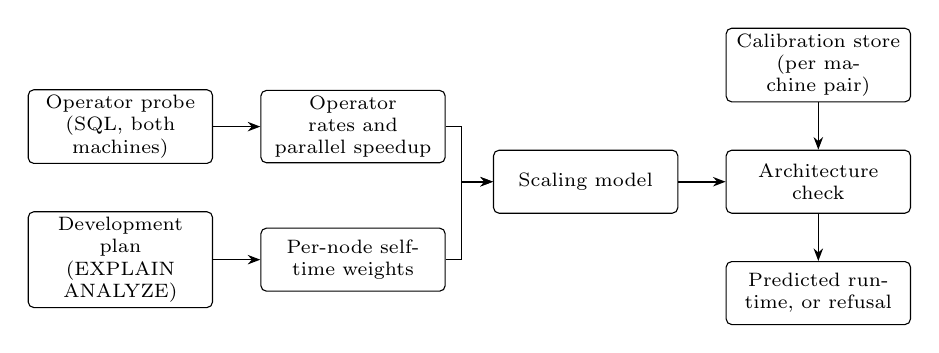
\begin{tikzpicture}[
  box/.style={draw, rounded corners=2pt, align=center, font=\scriptsize,
              minimum height=8mm, text width=22mm, inner sep=2pt},
  arr/.style={-{Stealth[length=1.6mm]}, semithick},
  node distance=6mm and 6mm]
\node[box] (probe) {Operator probe\\(SQL, both machines)};
\node[box, right=of probe] (rates) {Operator rates and parallel speedup};
\node[box, below=of probe] (plan) {Development plan\\(EXPLAIN ANALYZE)};
\node[box, right=of plan] (weights) {Per-node self-time weights};
\node[box, right=of rates, yshift=-7mm] (model) {Scaling model};
\node[box, right=of model] (guard) {Architecture check};
\node[box, above=of guard] (calib) {Calibration store\\(per machine pair)};
\node[box, below=of guard] (out) {Predicted runtime, or refusal};
\draw[arr] (probe) -- (rates);
\draw[arr] (plan) -- (weights);
\draw[arr] (rates.east) -- ++(2mm,0) |- (model.west);
\draw[arr] (weights.east) -- ++(2mm,0) |- (model.west);
\draw[arr] (model) -- (guard);
\draw[arr] (calib) -- (guard);
\draw[arr] (guard) -- (out);
\end{tikzpicture}
\caption{Overview of the CETP prediction pipeline}
\label{fig:pipeline}
\end{figure}

\subsection{First Design and Why It Was Replaced}
\label{sec:first}

The first design factored a runtime into the work a query asks for and the
rate at which a machine does that work. The work was a vector of planner
statistics. The machine was a pair of figures, STREAM-triad bandwidth and
OpenMP floating-point throughput. A random forest estimated whether a query
was limited by compute, bandwidth or input/output, and the scaling factor was
either a weighted combination of the two hardware ratios or the output of a
gradient-boosted regressor.

Three measurements ended it. The two hardware figures collapsed onto one
principal component carrying 97.9\% of their variance. The full estimator was
statistically indistinguishable from its simplest term
(Section~\ref{sec:legacy}). And predicting the cloud instances from a laptop
was worse than assuming the two were identical. We kept the factorisation and
replaced both halves of it.

\subsection{Operator Capability Probe}

The probe creates two synthetic tables, of two million and four hundred
thousand rows, and runs one statement per axis under \texttt{EXPLAIN ANALYZE}:
\begin{itemize}
\item \textbf{seqscan}: a filtered sequential scan;
\item \textbf{hashjoin}: building and probing a hash table;
\item \textbf{sort}: an in-memory sort;
\item \textbf{hashagg}: hash aggregation;
\item \textbf{nestloop}: an indexed nested-loop lookup, which exercises random
access;
\item \textbf{parallel scan}: the sequential scan repeated with three parallel
workers.
\end{itemize}
Each serial axis yields a rate $r_M(o)$ in tuples per second for machine $M$
and operator $o$. The sixth statement yields the parallel speedup
\begin{equation}
\sigma_M = \frac{r_M(\text{parallel scan})}{r_M(\text{seqscan})},
\end{equation}
which is the factor by which the machine really accelerates a scan when
PostgreSQL parallelises it.

Several settings are pinned so that two signatures are comparable. Just-in-time
compilation is off. The working-memory limit is fixed at 64\,MB on every
machine, because sort and hash rates depend on it strongly and a probe that
inherited each server's own setting would mix capability with configuration.
Each statement is repeated nine times, the parallel one eleven times, with
the first repetition discarded. The rates are instrumented rates and mean
nothing in isolation. They are only ever used as a ratio between two machines
measured the same way.

\subsection{Decomposing the Development Plan}

The development plan is walked node by node. The self-time of a node is its
total time less that of its children, and each node type is mapped to one of
the five axes. Control nodes such as Gather and Limit map to none, and their
time is tracked as an unmapped share. On the grid that share averaged 0.3\%
of query time.

One detail turned out to matter a great deal. Under a Gather node, PostgreSQL
reports each node's time averaged over the leader and its workers, so the
self-times in the parallel part of a plan add up to processor time and not to
elapsed time. On one parallel query the sum was 2.85 times the elapsed time.
We therefore divide the self-time of every node under a Gather by the
development machine's own speedup $\sigma_D$ before normalising. With $\pi
\in \{0,1\}$ marking whether a node runs under a Gather, the weights are
\begin{equation}
w_{o,\pi} = \frac{\tau_{o,\pi}}{\sum_{o',\pi'} \tau_{o',\pi'} + \tau_{\varnothing}},
\qquad
\tau_{o,\pi} = \sum_{n \in (o,\pi)} \frac{\text{self}(n)}{\sigma_D^{\,\pi}},
\end{equation}
where $\tau_{\varnothing}$ is the unmapped time. The weights and the unmapped
share $w_{\varnothing}$ sum to one.

\subsection{Scaling Model}

Each share of the development runtime is scaled by the capability ratio for
its operator. A parallel node runs at the per-worker rate multiplied by the
speedup, so its ratio carries both machines' speedups:
\begin{equation}
\rho_{o,\pi} = \frac{r_D(o)\,\sigma_D^{\,\pi}}{r_P(o)\,\sigma_P^{\,\pi}} .
\end{equation}
The predicted scaling factor is
\begin{equation}
\hat{s} = \sum_{o,\pi} w_{o,\pi}\,\rho_{o,\pi} \;+\; w_{\varnothing}\,\bar{\rho},
\label{eq:model}
\end{equation}
where $\bar{\rho}$ is the geometric mean of the ratios that were used, so that
unmapped work is assumed to scale like a typical operator. The predicted
production runtime is $\hat{t}_P = c \cdot \hat{s} \cdot t_D$, with $c$ the
calibration factor of Section~\ref{sec:calib}, equal to one when no
calibration exists. The model has no fitted parameters. Algorithm~\ref{alg:predict}
gives the complete procedure.

\begin{algorithm}[t]
\caption{Predict the production runtime of a query}
\label{alg:predict}
\begin{algorithmic}[1]
\State Load probe signatures of $D$ and $P$; reject either if flagged unreliable
\State Capture the plan of query $Q$ on $D$ with EXPLAIN (ANALYZE, BUFFERS, FORMAT JSON)
\State Compute node self-times; mark nodes under a Gather as parallel
\State Divide parallel self-times by $\sigma_D$ and normalise to weights $w_{o,\pi}$, $w_{\varnothing}$
\For{each $(o,\pi)$ with non-zero weight}
  \State $\rho_{o,\pi} \gets r_D(o)\,\sigma_D^{\pi} \,/\, \big(r_P(o)\,\sigma_P^{\pi}\big)$
\EndFor
\State $\hat{s} \gets \sum w_{o,\pi}\,\rho_{o,\pi} + w_{\varnothing}\,\bar{\rho}$
\State $c \gets$ stored calibration for the pair $(D,P)$, or $1$ if none
\If{architectures of $D$ and $P$ differ \textbf{and} no calibration is stored}
  \State \Return refusal, with a request to measure calibration queries on $P$
\EndIf
\State \Return $c \cdot \hat{s} \cdot t_D$, together with the unmapped share
\end{algorithmic}
\end{algorithm}

Two further terms are implemented but not evaluated here, and we make no claim
for them. One scales each operator by the ratio of rows it would process when
production holds more data than development. Every environment in this study
holds identical data, so the term was only ever exercised at a ratio of one.
The other obtains the plan from production with a plain EXPLAIN, which costs
no execution, and forces it on the development machine, so that a difference
in plan choice cannot contribute to the error. No query changed plan anywhere
in the grid, so this too could not be tested.

\subsection{Calibration}
\label{sec:calib}

If the probe misjudges a machine by a constant factor, a constant correction
removes the error. For each ordered pair of machines the system stores the
predicted and observed scaling factors of every query that has been measured
on the target, and sets
\begin{equation}
c = \operatorname{median}_{i}\left(\frac{s_i}{\hat{s}_i}\right).
\end{equation}
The median is used and not the mean, because with few observations a single
badly predicted query drags a mean a long way. A correction built from fewer
than three observations is reported as provisional, for a reason given in
Section~\ref{sec:calibresult}. Only the two scaling factors and a query
identifier are stored; no query text, literal or plan leaves the machine.

A correction belongs to one pair. It absorbs the scale error of one target
machine and says nothing about a different one. Accuracy therefore improves
with the number of queries measured on a given target, and we do not claim
that it improves with the number of machines a deployment has seen.

\subsection{Architecture Check}

When the two signatures were measured on different instruction sets and no
calibration is stored for the pair, the system returns a refusal and not a
number. Section~\ref{sec:crossisa} shows why: in that configuration the
uncalibrated model was about three times worse than assuming the two machines
are identical. A tool that returns a confident figure there does harm.

\subsection{Concurrency as an Input}

Everything above describes a query running alone. Runtime under $N$
simultaneous clients is modelled as $t(N) = t(1)\,N^{e}$, where the exponent
$e$ is the elasticity of the query. The caller supplies $N$, and may supply
$e$ if it has been measured. Section~\ref{sec:concurrency} explains why $e$
is an input and is not predicted.

\subsection{Implementation}

The system is a Python package with a command-line interface, and a Visual
Studio Code extension that runs a prediction on the SQL file open in the
editor. Plans are obtained through PostgreSQL, and the analysis uses NumPy
and pandas. Plan parsing was checked against PostgreSQL 14, 15, 17 and 18,
all of which parse without unmapped node types; versions 13 and 16 were not
tested.

\section{Results and Discussions}

Uncalibrated predictions have no fitted parameters, so there is nothing to
overfit and their error on all pairs is their held-out error. Calibrated
predictions are scored only on queries that were not used to fit the
correction. Differences between predictors are tested with a paired
bootstrap that resamples whole queries, with 95\% intervals.

\subsection{What the Model Needs: An Ablation on the Grid}
\label{sec:ablation}

Table~\ref{tab:ablation} and Fig.~\ref{fig:ablation} compare seven predictors
on the 1232 grid pairs. The first four cannot see parallelism: the naive
baseline, a single scalar taken from the scan rate, a single scalar taken as
the geometric mean over all five axes, and the per-operator model with the
parallel term removed. All four sit between 67\% and 73\%, within about six
points of the baseline and far from the three that have a parallel term.
Measuring five operators carefully and weighting them by where the time went
buys at most a few points by itself.

\begin{table}[t]
\centering
\caption{Prediction error on the container grid (1232 pairs)}
\label{tab:ablation}
\begin{tabular}{lcc}
\toprule
Predictor & MAPE (\%) & MdAPE (\%) \\
\midrule
Naive (production equals development) & 72.52 & 36.78 \\
Single scalar, scan rate & 70.98 & 34.64 \\
Single scalar, geometric mean of axes & 66.97 & 34.07 \\
Per-operator, no parallel term & 69.00 & 34.30 \\
\midrule
Single scalar, parallel term on whole query & 30.15 & 21.03 \\
Single scalar, parallel term on parallel nodes & 22.23 & 18.14 \\
Per-operator, parallel term on parallel nodes (CETP) & 22.41 & 18.34 \\
\bottomrule
\end{tabular}
\end{table}

\begin{figure}[t]
\centering
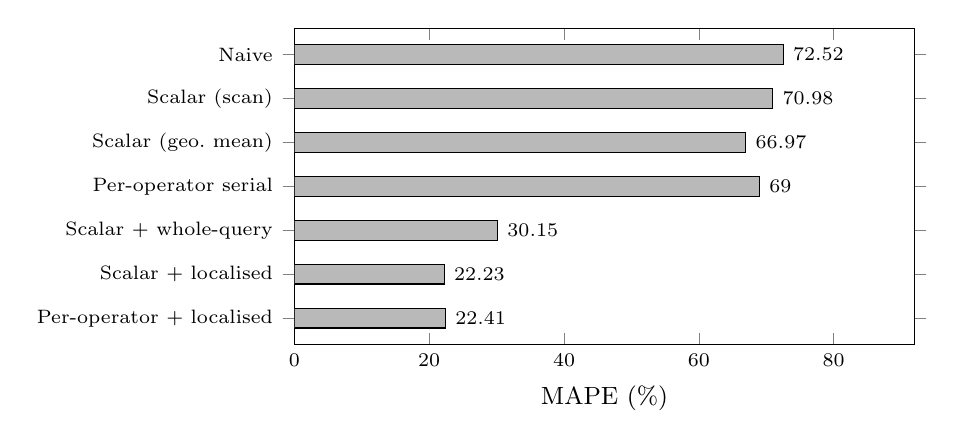
\begin{tikzpicture}
\begin{axis}[
  xbar, width=0.78\textwidth, height=5.6cm,
  xmin=0, xmax=92, xlabel={MAPE (\%)},
  symbolic y coords={G,F,E,D,C,B,A},
  ytick=data,
  yticklabels={Per-operator + localised,Scalar + localised,Scalar + whole-query,
               Per-operator serial,Scalar (geo.\ mean),Scalar (scan),Naive},
  yticklabel style={font=\scriptsize},
  xlabel style={font=\small}, tick label style={font=\scriptsize},
  nodes near coords, nodes near coords style={font=\scriptsize},
  bar width=7pt, enlarge y limits=0.1]
\addplot[fill=gray!55, draw=black] coordinates
  {(22.41,G) (22.23,F) (30.15,E) (69.00,D) (66.97,C) (70.98,B) (72.52,A)};
\end{axis}
\end{tikzpicture}
\caption{Error of each predictor on the container grid. The four predictors
without a parallel term stay within six points of the naive baseline.}
\label{fig:ablation}
\end{figure}

The reason is visible in the probe output. Across the eight cells no serial
rate varied by more than a factor of 1.39, while the parallel speedup ranged
from 0.76 to 2.70, a factor of 3.57. A CPU quota does not slow a single
worker, which needs only one core. What it changes is whether three workers
run side by side or take turns. Ninety-one percent of the pairs involve a
parallel plan, so that is where the runtime difference lives.

Adding the speedup ratio as a multiplier on the whole query brings the error
from 66.97\% to 30.15\%. Applying it only to the nodes under a Gather brings
it to 22.23\%, and that step is significant: the paired difference is 7.92
points with an interval of [1.45, 16.31].

The last comparison is the one we did not expect. The full per-operator model
scores 22.41\%. A single scalar with the parallel term placed on the right
nodes scores 22.23\%. The paired difference is $-0.17$ points with an
interval of [$-0.49$, $+0.10$], which includes zero. On this grid the
per-operator detail adds nothing that can be measured, and the useful
knowledge is which part of the plan runs in parallel. Against the naive
baseline the model's gain is 50.11 points, with an interval of [39.13,
62.48].

The five serial axes are less collinear than the old two-figure signature
but are still partly redundant. Their first principal component carries
72.4\% of the variance, their mean absolute pairwise correlation is 0.65, and
three components are needed to reach 95\%, against 97.9\% on a single
component for the old signature. Eight cells on one host are too few to say
more than that the signature carries some independent information. The grid
does not move the serial axes far enough for any extra dimension to change a
prediction, and we do not claim that it has more than three effective
dimensions.

\subsection{From a Laptop to Same-Architecture Targets}

The grid result is symmetric, with every cell predicting every other. The
case the system is built for is one-directional: the laptop itself as the
development machine. Table~\ref{tab:same} gives the result for the seven grid
cells used as targets.

\begin{table}[t]
\centering
\caption{Laptop to same-architecture targets (22 queries each)}
\label{tab:same}
\begin{tabular}{lcc}
\toprule
Target (CPU limit, memory limit) & Naive MAPE (\%) & CETP MAPE (\%) \\
\midrule
1 CPU, 1\,GB & 62.58 & 23.47 \\
1 CPU, 3\,GB & 59.78 & 31.26 \\
2 CPU, 3\,GB & 22.17 & 22.15 \\
4 CPU, 1\,GB & 32.41 & 36.00 \\
4 CPU, 3\,GB & 32.70 & 36.40 \\
8 CPU, 1\,GB & 30.84 & 33.42 \\
8 CPU, 3\,GB & 21.27 & 22.49 \\
\midrule
All seven (154 pairs) & 37.39 & 29.31 \\
\bottomrule
\end{tabular}
\end{table}

Overall the model improves on the baseline by eight points. The table shows
where those points come from, and it would be misleading to hide it. On the
two single-CPU targets, where capability differs sharply from the laptop, the
error falls from about 60\% to between 23\% and 31\%. On the four- and
eight-CPU targets, which behave much like the laptop, the baseline is already
right and the model is one to four points worse. The model earns its place
when the machines differ and costs a little when they do not.

The residual has a direction. The model over-predicts on six of the seven
targets, and the amount of over-prediction rises with the share of a query's
time that goes to reading data beyond the buffer pool (Spearman correlation
$+0.302$). The probe tables fit in memory, so nothing in the signature
describes storage. Section~\ref{sec:hygiene} describes our attempt to add
that axis.

\subsection{Across an Instruction-Set Boundary}
\label{sec:crossisa}

Table~\ref{tab:x86} gives the same experiment with the four x86 machines as
targets. The baseline is good here, about 21\%, because these machines happen
to run the workload at close to the laptop's speed. The model is not good. It
scores between 66\% and 73\% on every one of the four, and 68.92\% overall.

\begin{table}[t]
\centering
\caption{Laptop (arm64) to x86 targets: error and median scaling factor}
\label{tab:x86}
\begin{tabular}{lcccc}
\toprule
 & \multicolumn{2}{c}{MAPE (\%)} & \multicolumn{2}{c}{Median scaling} \\
\cmidrule(lr){2-3}\cmidrule(lr){4-5}
Target & Naive & CETP & Actual & Predicted \\
\midrule
X1 & 22.75 & 67.26 & 1.126 & 1.795 \\
X2 & 21.79 & 66.15 & 1.077 & 1.644 \\
X3 & 21.00 & 69.44 & 1.066 & 1.660 \\
X4 & 21.41 & 72.84 & 1.044 & 1.667 \\
\midrule
All four (88 pairs) & 21.74 & 68.92 & & \\
\bottomrule
\end{tabular}
\end{table}

Four machines giving the same answer rules out noise, so we looked for the
mechanism. The natural suspicion is that a different instruction set changes
the relative cost of operators, making a sort comparatively dearer on one
chip than on another. If that were so, the five per-axis ratios between the
laptop and an x86 machine would be widely spread. They are not. The largest
ratio divided by the smallest is between 1.20 and 1.27 on the four machines.
For comparison, the worst pair of cells inside the single-host grid has a
spread of 1.37. Crossing the architecture boundary disturbs the operator mix
less than changing a resource limit on one machine does.

What fails to transfer is the level. The right half of Table~\ref{tab:x86}
shows it plainly. The probe implies that the x86 machines are 1.64 to 1.80
times slower than the laptop. The real workload ran 1.04 to 1.13 times
slower. Every ratio is inflated by roughly the same factor, so the shape of
the prediction is right and its scale is wrong. Tuples per second on a small
synthetic table is not a unit that carries across microarchitectures. This
is the same defect that sank the floating-point signature, and measuring six
SQL-level figures in place of two benchmark figures did not remove it.

\subsection{Calibration}
\label{sec:calibresult}

A constant scale error is exactly what the correction of
Section~\ref{sec:calib} removes. Figure~\ref{fig:calib} shows the error as a
function of the number of queries $k$ measured on the target. For each $k$ we
draw the queries at random, fit the correction, and score the remaining
queries, averaging over 200 draws per target.

\begin{figure}[t]
\centering
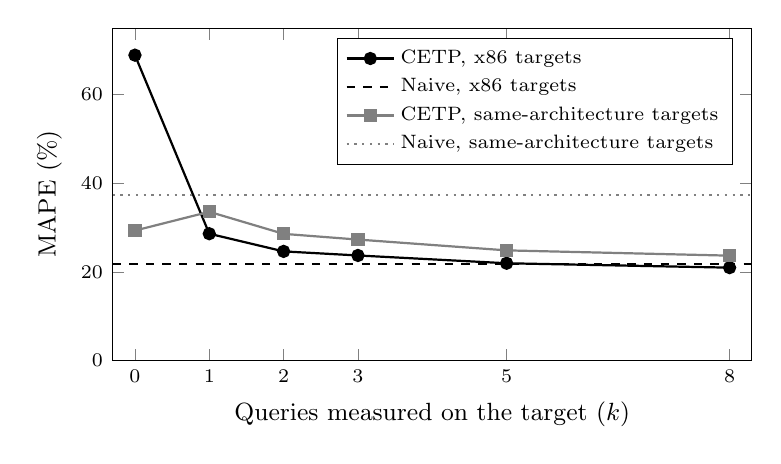
\begin{tikzpicture}
\begin{axis}[
  width=0.80\textwidth, height=5.8cm,
  xlabel={Queries measured on the target ($k$)}, ylabel={MAPE (\%)},
  xmin=-0.3, xmax=8.3, ymin=0, ymax=75,
  xtick={0,1,2,3,5,8},
  label style={font=\small}, tick label style={font=\scriptsize},
  legend style={font=\scriptsize, at={(0.97,0.97)}, anchor=north east},
  legend cell align=left]
\addplot[mark=*, thick] coordinates
  {(0,68.92) (1,28.60) (2,24.61) (3,23.69) (5,21.93) (8,20.94)};
\addlegendentry{CETP, x86 targets}
\addplot[dashed, thick, domain=-0.3:8.3] {21.74};
\addlegendentry{Naive, x86 targets}
\addplot[mark=square*, thick, gray] coordinates
  {(0,29.31) (1,33.55) (2,28.57) (3,27.28) (5,24.84) (8,23.65)};
\addlegendentry{CETP, same-architecture targets}
\addplot[dotted, thick, gray, domain=-0.3:8.3] {37.39};
\addlegendentry{Naive, same-architecture targets}
\end{axis}
\end{tikzpicture}
\caption{Error against the number of calibration queries measured on the
target machine}
\label{fig:calib}
\end{figure}

On the x86 targets one measured query takes the error from 68.92\% to
28.60\%, three take it to 23.69\% and five to 21.93\%. That is level with the
naive baseline of 21.74\% and not clearly below it at any $k$ we tried. The
honest summary is that across an architecture boundary, calibration repairs
the model, and the repaired model then tells the developer about as much as
the calibration queries alone would have.

On the same-architecture targets the picture differs in two ways. The model
is ahead of the baseline before any calibration, and calibration widens the
gap, to 24.84\% against 37.39\% at five queries. But a single query makes
things worse, 33.55\% against 29.31\% uncalibrated. When the uncalibrated
model is already reasonable, one unlucky query is enough to push every other
prediction the wrong way. This is why the system labels a correction built on
fewer than three observations as provisional.

\subsection{The Earlier Two-Figure Model}
\label{sec:legacy}

The cloud dataset supports two findings that hold regardless of what replaced
the model.

Under leave-one-machine-out cross-validation on 420 pairs, the analytical
roofline estimator scores 21.61\% against 23.05\% for scaling by the
bandwidth ratio alone. The improvement of 1.44 points has an interval of
[0.32, 2.56] and is significant. But scaling by the compute ratio alone, with
no classifier and no weighting, scores 20.06\%. The difference between that
and the full estimator has an interval of [$-0.41$, $+3.51$]. The gain came
from choosing compute over bandwidth as the signal, and the classifier and
weighting built on top contributed nothing measurable. The bottleneck
classifier itself reached a macro-averaged F1 of only 0.375 once a
buffer-accounting error in the dataset was corrected, and never once
identified the input/output class. The learned regressor behaved as fitted
models do: 17.29\% when the target machine was in its training data and
26.86\% when it was not.

The compute signal mattered only in its multi-core form. Measured on a single
core it correlated with the observed scaling factor at $+0.213$, the wrong
sign. Measured across all cores it correlated at $-0.691$. PostgreSQL spreads
an analytical query over several workers, so the throughput that governs
runtime is that of the whole machine. The parallel term of the present model
is the same observation made precise.

The second finding is a ceiling. On each cloud instance the true scaling
factor from the laptop varies by a factor of 18 to 43 across queries. Any
predictor that multiplies by one number per machine pair, however well that
number is chosen, cannot go below 59.7\% MAPE on those pairs. The best
calibrated single-factor result we measured was 55.9\% on a held-out subset,
which scores a different set of queries and lands in the same region. Getting past it requires a term that
varies by query, which is what the plan weights provide.

\subsection{Concurrency}
\label{sec:concurrency}

We ran all 22 queries on the laptop with 1, 2, 4 and 8 simultaneous clients.
The power law $t(N) = t(1)\,N^{e}$ fits well, with a median $R^2$ of 0.944.
The elasticity $e$ has a median of 0.734 and ranges from 0.286 to 0.984, and
the largest slowdown at eight clients was a factor of 8.57. That is larger
than any hardware effect in this study.

We then tried to predict each query's elasticity from its plan, leaving one
query out at a time. Plan features gave a mean absolute error of 0.191. Using
the median of the other queries gave 0.167. The plan carries no usable signal
about how a query responds to load. Table~\ref{tab:conc} shows the
consequence for runtime at eight clients. A default exponent roughly halves
the error of ignoring load, and knowing the query's own exponent would cut it
to under 7\%. Concurrency is therefore an input the caller supplies, with a
default that helps and a measured value that helps far more.

\begin{table}[t]
\centering
\caption{Runtime error at eight concurrent clients, by treatment of load}
\label{tab:conc}
\begin{tabular}{lc}
\toprule
Treatment & MAPE (\%) \\
\midrule
Ignore concurrency & 73.79 \\
Median elasticity for every query & 41.81 \\
Elasticity predicted from plan features & 42.64 \\
Each query's own measured elasticity & 6.72 \\
\bottomrule
\end{tabular}
\end{table}

\subsection{What Went Wrong with the Instrument}
\label{sec:hygiene}

Several figures in earlier drafts of this work were wrong because of the
probe and not the model. We list the cases because probe repeatability is
rarely reported and here it changed conclusions.

\begin{itemize}
\item \textbf{The probe was too short.} With small tables the parallel scan
finished in 18\,ms, so worker start-up was a large part of the measurement.
The speedup came back with a coefficient of variation of 0.50, including a
value of 1.81 on a machine limited to one CPU, which is impossible. With
tables large enough for each run to take a few hundred milliseconds, the
same machine reports about 0.8: three workers sharing one core are slower
than one worker alone.
\item \textbf{The validity check tested the wrong thing.} An early check
rejected a signature when its repetitions varied too much. The reported rate
is a median, and the median of the parallel axis was reproducible to within
a few percent even when individual runs were not. The check discarded half
the grid before it was changed to test the stability of the median.
\item \textbf{The machine was not idle.} Probing while other work was running
cut the measured parallel speedup roughly in half. A signature taken under
contention describes the contention. The system now flags such a signature
and refuses to use it.
\item \textbf{The storage axis did not measure storage.} To address the
residual bias, we added a scan over a table larger than the buffer pool.
Across the grid its rate tracked the CPU limit (Spearman 0.762) more closely
than the memory limit (0.548). It was measuring sustained throughput under a
CPU quota, not disk. The axis is recorded but excluded from the model.
\end{itemize}

\section{Conclusion and Future Works}

This paper presented CETP, which predicts the production runtime of a
PostgreSQL query from a plan captured on the developer's machine, using a
capability signature measured in SQL. On a grid of containers the model
reduced the error from 72.52\% to 22.41\%, and from a laptop to
same-architecture targets from 37.39\% to 29.31\%. Nearly all of that comes
from one term, the ratio of the two machines' parallel speedups applied to
the nodes that actually run in parallel. Across an instruction-set boundary
the uncalibrated model was three times worse than doing nothing, on four
machines out of four. The relative operator mix carried across; the absolute
scale did not. Five measured queries restored the error to about 22\%, which
matches the baseline and does not beat it. The system refuses to give an
uncalibrated cross-architecture answer.

The limitations are real and we list them plainly. The workload is 22 queries
at one scale factor. The grid varies resource limits on one physical host and
so cannot say anything about different cache hierarchies. Development and
production always held identical data, so the row-count term is untested, and
no plan ever differed between environments, so plan forcing is untested as
well. Nothing in the signature measures storage, and that is the diagnosed
source of the remaining bias. All accuracy figures are for a query running
alone. Within one architecture the gain is concentrated in targets that
differ from the development machine, and on similar machines the baseline is
slightly better. CETP is a way to catch a query that will be several times
slower in production. It does not replace a benchmark on a staging server
when a decision rests on an absolute figure.

Future work follows from those gaps. A storage axis needs a probe table
larger than physical memory, which was beyond the disk available to us. The
scale error across architectures might be reduced by anchoring the probe to a
few real queries in place of synthetic tables, or by pooling corrections
across machines of the same family; neither has been shown. A larger scale
factor would exercise the row-count term, and environments with different
indexes and planner settings would exercise plan forcing. Finally, the
elasticity of a query under load has to be measured today. Whether it can be
predicted from features of the concurrent mix, since it cannot be predicted
from the plan, is an open question.

\begin{thebibliography}{99}

\bibitem{akdere}
Akdere, M., \c{C}etintemel, U., Riondato, M., Upfal, E., Zdonik, S.B. (2012).
Learning-based query performance modeling and prediction. In:
\emph{Proceedings of the IEEE International Conference on Data Engineering
(ICDE)}, pp. 390--401.

\bibitem{duggan}
Duggan, J., \c{C}etintemel, U., Papaemmanouil, O., Upfal, E. (2011).
Performance prediction for concurrent database workloads. In:
\emph{Proceedings of the ACM SIGMOD International Conference on Management of
Data}, pp. 337--348.

\bibitem{efron}
Efron, B., Tibshirani, R.J. (1993). \emph{An Introduction to the Bootstrap}.
Chapman and Hall, New York.

\bibitem{ganapathi}
Ganapathi, A., Kuno, H., Dayal, U., Wiener, J.L., Fox, A., Jordan, M.,
Patterson, D. (2009). Predicting multiple metrics for queries: Better
decisions enabled by machine learning. In: \emph{Proceedings of the IEEE
International Conference on Data Engineering (ICDE)}, pp. 592--603.

\bibitem{hilprecht}
Hilprecht, B., Binnig, C. (2022). Zero-shot cost models for out-of-the-box
learned cost prediction. \emph{Proceedings of the VLDB Endowment}, 15(11),
2361--2374.

\bibitem{leis}
Leis, V., Gubichev, A., Mirchev, A., Boncz, P., Kemper, A., Neumann, T.
(2015). How good are query optimizers, really? \emph{Proceedings of the VLDB
Endowment}, 9(3), 204--215.

\bibitem{marcus}
Marcus, R., Negi, P., Mao, H., Zhang, C., Alizadeh, M., Kraska, T.,
Papaemmanouil, O., Tatbul, N. (2019). Neo: A learned query optimizer.
\emph{Proceedings of the VLDB Endowment}, 12(11), 1705--1718.

\bibitem{mccalpin}
McCalpin, J.D. (1995). Memory bandwidth and machine balance in current high
performance computers. \emph{IEEE Technical Committee on Computer
Architecture Newsletter}, pp. 19--25.

\bibitem{postgres}
The PostgreSQL Global Development Group. (2024). PostgreSQL documentation:
Using EXPLAIN. Available at: https://www.postgresql.org/docs/

\bibitem{sun}
Sun, J., Li, G. (2019). An end-to-end learning-based cost estimator.
\emph{Proceedings of the VLDB Endowment}, 13(3), 307--319.

\bibitem{tpch}
Transaction Processing Performance Council. (2021). TPC Benchmark H (Decision
Support) Standard Specification, Revision 3.0. TPC.

\bibitem{williams}
Williams, S., Waterman, A., Patterson, D. (2009). Roofline: An insightful
visual performance model for multicore architectures. \emph{Communications of
the ACM}, 52(4), 65--76.

\bibitem{wu}
Wu, W., Chi, Y., Zhu, S., Tatemura, J., Hac{\i}g\"{u}m\"{u}\c{s}, H.,
Naughton, J.F. (2013). Predicting query execution time: Are optimizer cost
models really unusable? In: \emph{Proceedings of the IEEE International
Conference on Data Engineering (ICDE)}, pp. 1081--1092.

\end{thebibliography}

\end{document}
